%\documentclass[a4paper,11pt]{report}
\documentclass[a4paper,11pt]{article}
\usepackage[utf8]{inputenc}
\usepackage[italian]{babel}
\usepackage{amsmath,amssymb, enumerate, indentfirst, booktabs, listings, colortbl, tabularx, graphicx, url}
\usepackage{emp} 

% include the web pages examined in the bibliography
\makeatletter
\let\@orig@endthebibliography\endthebibliography
\renewcommand\endthebibliography{
\xdef\@kept@last@number{\the\c@enumiv}
\@orig@endthebibliography}
\newenvironment{thesitography}[1]
%{\def\bibname{Siti consultati}% Classe book o report
{\def\refname{Siti consultati}% Classe article
\thebibliography{#1}%
\setcounter{enumiv}{\@kept@last@number}%
}
	{\@orig@endthebibliography}
\makeatother

\definecolor{orange}{rgb}{1,0.5,0}
\lstnewenvironment{java}{\lstset{basicstyle=\ttfamily,
stepnumber=2, numbersep=5pt, language=java, %frame=shadowbox, 
keywordstyle=\color{red}\bfseries, commentstyle=\color{blue}, 
stringstyle=\color{orange}}}{}

\newcolumntype{G}{>{\columncolor[gray]{0.8}}c}

\setlength{\parindent}{3mm}
\newcommand{\grammarindent}[1][1]{\hspace*{#1\parindent}\ignorespaces} 


% set margin
\usepackage{vmargin}
\setpapersize{A4}
\setmarginsrb{25mm}{5mm}{25mm}{8mm}
             {0mm}{10mm}{0mm}{10mm}


\title{\bf{Implementazione di un dimostratore di teoremi per risoluzione}}
\author{Enrico Scapin vr353597}
\date{\today}

\begin{document}

\maketitle

\small
\section{Introduzione}
Uno degli obiettivi del ragionamento automatico consiste nel cercare di costruire \emph{Dimostratori Automatici di Teoremi} al fine di ottenere meccanismi automatizzabili per asserire, a partire da un insieme di assunzioni $H$, la validità o meno di una determinata congettura $\varphi$. Più formalmente:
\[ H \models \varphi \]
I dimostratori automatici tipicamente procedono in maniera refutazionale in quanto ogni formula è valida se e solo se la sua negazione è insoddisfacibile. Quindi, riferendoci al sequente sopra:
\[ H \models \varphi \Longleftrightarrow H \cup \lbrace\neg \varphi\rbrace \text{ è insoddisfacibile} \]
Da questa considerazione possiamo quindi cercare di costruire una procedura che, se dimostra l'insoddisfacibilità di $H \cup \lbrace\neg \varphi\rbrace$, allora $ H \models \varphi $ è valido, altrimenti, se ne dimostra la sua soddisfacibilità, il modello che lo soddisfa costituirà il controesempio alla validità di $ H \models \varphi $.\par
Siamo interessati a dimostrare formule espresse in Logica del Primo Ordine\footnote{\emph{FOL}, First Order Logic} in quanto, al contrario della logica proposizionale, essa è sufficientemente espressiva da poter modellare una buona parte della nostra conoscenza. Utilizzando questo linguaggio però il problema della validità non è più decidibile bensì semidecidibile: infatti se l'insieme $H \cup \lbrace\neg \varphi\rbrace $ è insoddisfacibile allora la procedura terminerà sempre con la risposta corretta, mentre se esso è soddisfacibile non è detto che la procedura termini. \par
La semidecidibilità deriva direttamente dal \emph{Teorema di Herbrand} che afferma che un insieme finito $S$ di clausole in \emph{FOL} è soddisfacibile se e solo se esiste un insieme finito $S'$ di istanze ground (clausole in cui tutte le variabili sono istanziate ad una qualche costante) di clausole di $S$ tale che $S'$ è soddisfacibile. Quindi per dimostrare la soddisfacibilità di $S$ è necessario generare tutti gli insiemi $S'$ di istanze ground e dimostrarne la soddisfacibilità ma, se in $S$ si quantifica su insiemi infiniti, allora la cardinalità degli insiemi $S'$ da generare è anch'essa infinita.\par
Questo dimostratore prende in ingresso un insieme di clausole scritte in Forma Normale Congiunta\footnote{\emph{CNF}, Conjunctive Normal Form} e definite da una sintassi standard compatibile con frammento CNF senza uguaglianza della libreria \emph{TPTP} (vedi \cite{TPTP}). Si è quindi implementata una procedura di semi-decisione che, basata su un sistema di cinque regole di inferenza (di cui due di espansione e tre di contrazione), implementa un piano di ricerca denominato \emph{Ciclo della Clausola Data} (Given clause loop) che è uno standard alla base di molti dimostratori di insieme di formule in logica al primo ordine come Otter, E, Vampire, Gandalf etc.

%%%%%% Scelte progettuali implementative %%%%%%%%
\section{Scelte progettuali ed implementative}
L'elaborato è stato implementato utilizzando il linguaggio \emph{Java} in quanto il livello di astrazione è tale da permettere al programmatore di concentrarsi principalmente sulla progettazione dell'algoritmo ed, in particolare, su quali strutture dati sia meglio utilizzare. 
\subsection{Parser}
La scelta di \emph{Java} consente inoltre l'utilizzo di \emph{JavaCC}, uno strumento che ha permesso di effettuare sia il parsing delle formule sia quello degli argomenti che vengono passati da riga di comando: i due parser consistono in file con estensione \texttt{.jj} costituiti da un'unità di compilazione java e da una grammatica context-free di tipo \emph{LL(1)} le cui produzioni sono espresse in BNF (\emph{Backus–Naur Form}).
Per quanto riguarda il parsing degli argomenti la grammatica è molto semplice:
\\[1mm]
\begin{ttfamily}
\grammarindent SelectionStrategy $::=$  -fifo | -best$($<Numeric>$)?$ \\
\grammarindent SearchStrategy ~~~$::=$  -contr | -exp \\
\grammarindent LoopType $::=$ 	-o | -e\\
\grammarindent Time ~~~~$::=$ 	-time<Numeric>\\
\grammarindent FilePath $::=$ <Char>\\
\\[1mm]
\end{ttfamily}
I token \texttt{<Numeric>} e \texttt{<Char>} sono specificati dalle 
seguenti espressioni regolari:\\[1mm]
\begin{ttfamily}
\grammarindent Numeric $::=$ $($["0"-"9"]$)^+$\\
\grammarindent Char~~~ $::=$ $\widehat{}$["-","\textbackslash t"]$($ $\widehat{}$["\textbackslash t"]$)^*$\\[1.5mm]
\end{ttfamily}
Queste categorie indicano le possibilità con coi può essere eseguito il dimostratore implementato e sono documentate nel file README: si è deciso di utilizzare il parser per dare all'utente la possibilità di inserirli nell'ordine preferito ed inoltre solo il token \texttt{FilePath} è obbligatorio (in quanto consiste nella formula in input che deve essere dimostratata).
La configurazione di default degli argomenti in cui è prevista una scelta è la seguente:\\[1mm]
\begin{ttfamily}
\grammarindent SelectionStrategy $::=$  -best \\
\grammarindent SearchStrategy ~~~$::=$  -contr\\
\grammarindent LoopType $::=$ 	-o \\
\\[1mm]
\end{ttfamily}
Il significato semantico di ognuno di essi sarà poi spiegato successivamente.\par 
Per quanto riguarda invece il parsing del file contentente le formule, la grammatica corrisponde al frammento \emph{CNF} senza uguaglianza di quella di TPTP che può essere reperita in \cite{TPTPsyntax}.\par
Per quanto riguarda l'aspetto semantico è stato inserito del codice Java che si preoccupa di costruire ciascuna clausola, partendo dai suoi letterali e a loro volta dai loro termini, per poi inserirla nella struttura dati apposita. Il tipo di struttura dati dipende dal comando specificato dall'utente per il token \texttt{SelectionStrategy}: nel caso sia stato inserito \texttt{-best} la struttura dati è una coda di min priorità in cui l'ordinamento è definito dal numero di simboli che compongono ciascuna clausola, altrimenti nel caso sia stato inserito \texttt{-fifo} la struttura dati è una lista in cui le clausole vengono inserite nell'ordine in cui vengono lette.

\subsection{Bean Class}
La scelta dell'utilizzo di \emph{Java} ha permesso un minimo di progettazione orientata agli oggetti soprattutto delle cosidette classi bean\footnote{così si denotano le classi che logicamente contengono le informazioni da manipolare} e, in particolare, delle classi che definisco i termini (funzioni, variabili e costanti) e i letterali. 

\begin{figure}[h]
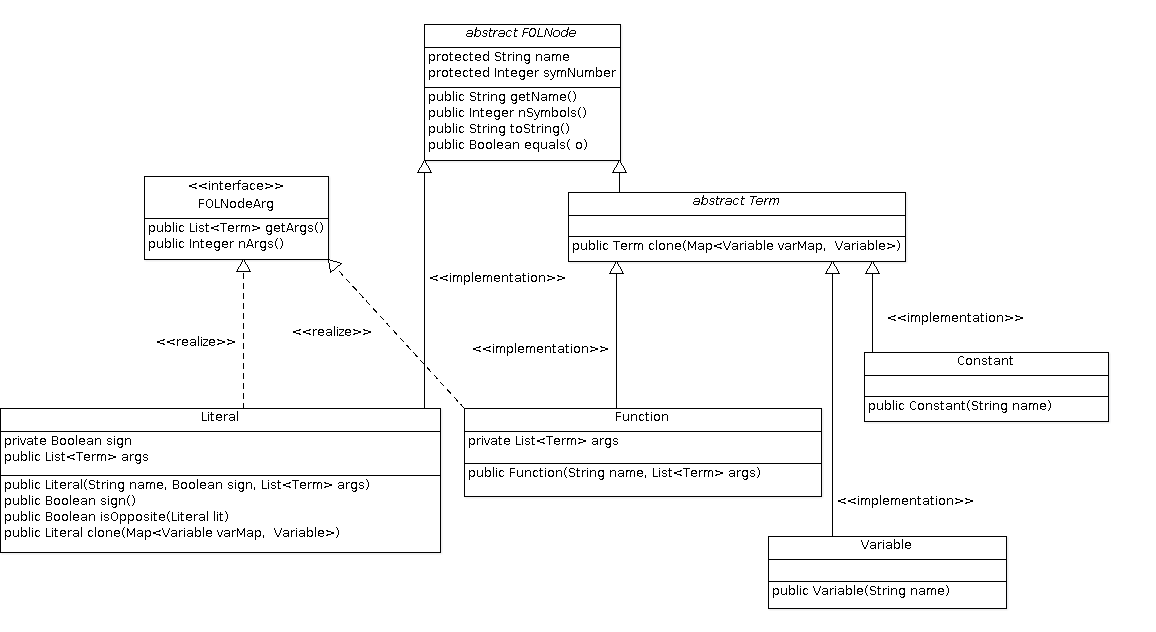
\includegraphics[width=1\columnwidth]{beanClassUML.png}
\caption{\small{UML delle bean class}}
\label{beanClassUML}
\end{figure}

Il diagramma UML visibile in Figura \ref{beanClassUML} rappresenta come è state progettate le classi: ovviamente è molto rilevante la classe astratta \texttt{Term}, che rappresenta un qualsiasi oggetto di tipo \texttt{Function}, \texttt{Variable} o \texttt{Constant}, in quanto è spesso necessario riferirsi ad una di esse indistintamente (come ad esempio quando si specificano gli argomenti di un letterale). Il metodo \texttt{clone(Map<Variable, Variable>)} presente sia nella classe \texttt{Term} sia nella classe \texttt{Literal} permette di clonare l'oggetto in questione restituendone un altro con la stessa struttura. Questo metodo si rivela essere molto importante quando è necessario generare una nuova clausola a partire da un'altra: infatti è sufficiente chiamare il metodo \texttt{clone} su ogni letterale che ricorsivamente clonerà anche i termini che compongono i suoi argomenti. Quando si crea un nuova clausola è però necessario mantenere inalterato il numero delle variabili in modo tale che tutte le occorrenze di ogni variabile nella vecchia clausola vengano rimpiazzate dalla stessa nuova variabile nella nuova: per far ciò è necessario avere una mappa che mantiene il collegamento tra il vecchio oggetto \texttt{Variable} con il nuovo se esso è già stato creato in precedenza in quanto quella determinata variabile è stata già incontrata in precedenza durante la clonazione. Alternativamente se quella variabile non è stata incontrata in precedenza allora è necessario crearne una nuova e inserire la coppia $(vecchia, nuova)$ all'interno della mappa. Se invece al posto di una variabile il metodo clone è chiamato su una costante, essa non verrà clonata (perché il set delle costanti deve rimanere sempre inalterato) bensì verrà ritornata la stessa.\par
Per quanto riguarda il metodo \texttt{toString} è da segnalare l'implementazione nella classe \texttt{Variable} in quanto, per differenziare le variabili diverse ma con lo stesso nome, si è scelto di concatenarci gli ultimi 3 caratteri del loro \emph{hash code} codificato in esadecimale.
Da notare infine il metodo \texttt{equals} che nel caso delle variabili ritorna \texttt{true} se e solo se sono lo stesso oggetto mentre nel caso delle costanti ritorna \texttt{true} se esse hanno lo stesso nome (e questo è consistente col fatto che le costanti sono le stesse per tutto l'insieme di clausole). Di conseguenza i metodi \texttt{equals} delle funzioni e dei letterali, dopo aver controllato l'uguaglianza dei segni e/o dei nomi, andranno in ricorsione sul termini che compongono i loro argomenti e solo se sono tutti uguali ritorneranno \texttt{true}.

\subsection{Core Class}

\begin{thebibliography}{9}
			\bibitem{deClercq: architectures} De Clercq J. (2002),
			\newblock "Single Sign On Architettures", \emph{Lecture Notes in Computer Science. Springer Verlag}.
\end{thebibliography}
\begin{thesitography}{9}
\bibitem{TPTP}
\url{http://www.cs.miami.edu/~tptp/}
\bibitem{TPTPsyntax}
\url{http://www.cs.miami.edu/~tptp/TPTP/SyntaxBNF.html}		
\end{thesitography}

\end{document}



